\documentclass[11pt, a4paper]{article}
%\usepackage[danish]{babel}
\usepackage{amsmath}
\usepackage[utf8]{inputenc}
%\usepackage{xfrac}
\usepackage{amsfonts}
\usepackage{amssymb}
\usepackage{tikz}
\usepackage{array}
\usepackage{cancel}
\usepackage{ulem}
\usepackage{graphicx}
\usepackage[a4paper]{geometry}
\usepackage{gauss}
%\usepackage{mathtools}
\usepackage{amsmath}
\usepackage{lastpage}
\usepackage{fancyhdr}
\usepackage{multirow}
\usepackage{listings}
\setlength{\headheight}{15.2pt}
\pagestyle{fancy}
\fancyhf{}
\lhead{Mads Anthony, MANA} %husk denne
\rhead{Side\ \thepage\ af\ \pageref{LastPage}} %husk 2 builds for dette!
%\usepackage[ansinew]{inputenc} 
\usepackage{enumerate}
%dot2tex loads
\usetikzlibrary{shapes}
\begin{document}
\author{Mads Anthony}
\section{Experiments}
\subsection{Setup}
With the background knowledge of neural oscillations and their possibly important role in doing modular tasks, it could be interesting to see how new methods that use these observations perform against other known modular methods.
\\
\\
In this section I therefore introduce two new methods that is based on neural oscillations, MiO-HyperNEAT and MaO-HyperNEAT which is explained in the beginning of this sections. Their results will be compared against a modular method by Schrum[ref] that is based in Hyper-NEAT and another simple network that doesn't have any modularity.
\subsection{MB-Hyper-NEAT [ref]}
As a comparison for how the new methods perform, I will be  using an extension to Hyper-NEAT called MB-Hyper-NEAT by Schrum[]. MB-Hyper-NEAT is inspired by the direct encoding MM-NEAT, which introduces methods to generate modules to NEAT. The idea with MB-Hyper-NEAT is to use multiple "brains" (MB) by encoding multiple networks on different substrates. In the group of MB-Hyper-NEAT these networks can be generated in different ways, however I will only be focusing on two of the methods: namely Multitask CPPNs and Preference Neurons.
\subsubsection{Multitask CPPNs [ref]}
Recall that a regular CPPN has one output to query weights and another output for bias. This setup is fine if we only want to encode one network, however for Multitask CPPN we are interested to encode multiple networks. Therefore Multitask CPPN introduces $ n $ extra pairs of weight/bias-outputs, that can be used to encode the same nodes on the substrate but with different weights and biases. This way Multitask CPPN's generate different networks, so that one network can be used for one task and another network for a different task. However when to switch between the different networks must still be specified by a human - which can be problematic as it require some insight into the domain and can also bias the final result. This problem is addressed in the other MB-HyperNEAT method using Preference Neurons.
\begin{figure}[!ht]
\centering
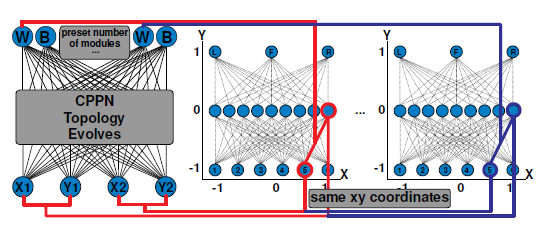
\includegraphics[scale=0.6]{MultitaskCPPN}
\caption{}
\end{figure}
\subsubsection{Preference Neurons [ref]}
This method builds upon multitasking CPPN, and introduces a way that let HyperNEAT discover when to switch between the different networks. This is done by having an extra output on the substrate network called a preference neuron. The preference neuron exist on each network, and the one with the heighest input is the network that get chosen. The connections weights to the preference neuron gets encoded by it's own output from the CPPN. An example can be seen in figure (x).
\begin{figure}[!ht]
\centering
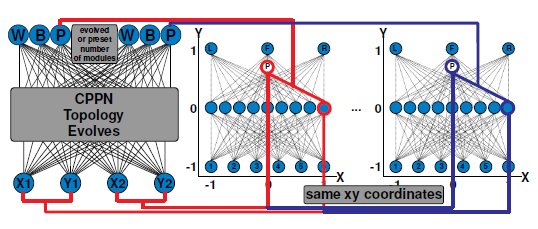
\includegraphics[scale=0.6]{PreferenceNeurons}
\caption{}
\end{figure}
\subsubsection{Microscopic Oscilliations HyperNEAT (MiO-HyperNEAT)}
The general idea with this method is to try and mimic the oscillation that happens on the microscopic level of the brain and use that to modularize the network. As mentioned earlier, the microscopic oscillations (MiO) is the firing patterns that take place for each neuron. To mimic this, MiO-HyperNEAT uses HyperNEAT together with SUPG to evolve oscillations for each hidden neuron placed on the substrate.
\\
\\
Along with the oscillation evolved for each hidden neuron the network on the substrate has an extra output that generate a \textit{Master Frequency}. The master frequency, isn't evolved using a SUPG, but is instead generated as a normal output (that if necessary can be modulated onto some pre-defined function - ex. sine function). The idea with the master frequency is to generate a frequency that is dependent on the environment, whereas the neuron oscillations only are determined by their position on the substrate.
\\
\\
Each hidden neuron then compare their oscillations with the master frequency, and if they are in synchrony they are enabled, and if not - they are disabled. One reason for this, is to let Hyper-NEAT try to discover frequencies that make part of the network be active at different times. Another reasons is that research (as mentioned earlier) points to certain oscillations be in synchrony for different task.
\\
\\
Since the total number of ways the hidden neurons can be active/disabled is $ 2^n $ it could in theory mean that Hyper-NEAT could discover $ 2^n $ modules - where $ n $ is the number of hidden neurons. A setup of the method can be seen in figure (x).
\begin{figure}[!ht]
\centering
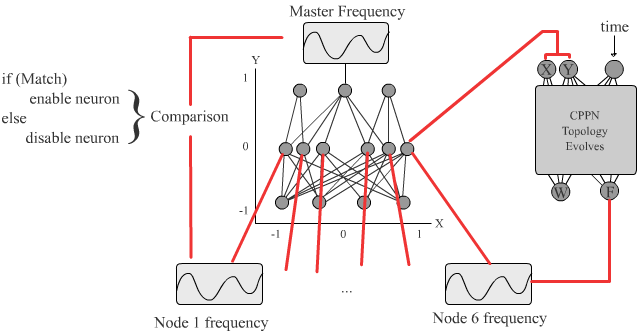
\includegraphics[scale=0.5]{MiO-HyperNEAT}
\caption{}
\end{figure}
\subsubsection{MaO-HyperNEAT}
\subsection{Experiment 1 - Recognizing time patterns}
\begin{center}
    \begin{tabular}{ | p{4cm} | l | l | l |}
    \hline
    Function & Image1 & Image2 & Error term ($ r^2 $) \\ \hline
    \begin{equation} f(x) =
    \begin{cases}
      0, & \text{if}\ x<0.5 \\
      1, & \text{otherwise}
    \end{cases} \nonumber \end{equation} &  \raisebox{-1\height}{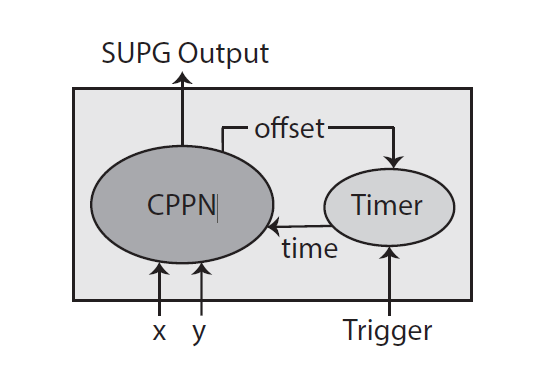
\includegraphics[scale=0.2]{SUPG}} &
\raisebox{-1\height}{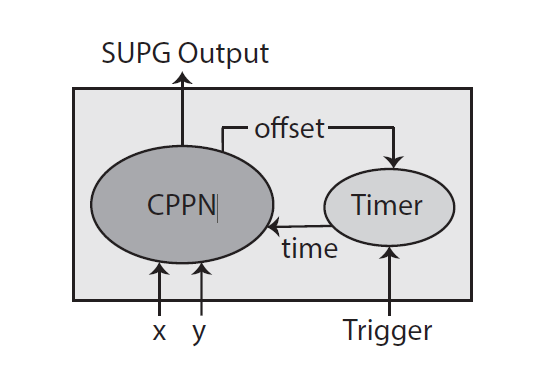
\includegraphics[scale=0.2]{SUPG}} &  
0.9
\\
    \hline
   \begin{equation} f(x) = sin(x) \nonumber \end{equation}  &
    &  &  \\
   \hline
   \begin{equation} f(x) = 3 \cdot sin(x+2) \nonumber \end{equation}  & & &  \\
   \hline
   \begin{equation} f(x) = gauss(x) \nonumber \end{equation}  & & &  \\
      \hline
    \end{tabular}
\end{center}
\subsection{Experiment 2 - Timely split task (Prey-Predator)}
Now that I've tested how good the SUPG is at recognizing different oscillations, it's time to test how well the two new methods perform on an actual problem that requires multitasking. To do this I've come up with a simple domain that has a very clear split between two different task. The domain is inspired by pac-man and consist of two task, one where the agent is a prey and another where it is the predator. A detailed explanation of the domain and the sensors is given in the beginning of this section, and is then followed by the results of each method. 
\subsubsection{Prey-Predator Domain}
The idea with this domain is to have a relatively simple domain that has a very clear split between two tasks. The switch happens in a timely manner to ensure the agent is forced to experience both tasks - unlike a environmental task, where the agent first has to "discover" the task based on for example a position in the domain.
\\
\\
The Prey-Predator domain consist of 1 agent and 3 enemies that are placed on a square board. The board is using a wrap-around design, so if you pass one of the edges you will appear on the opposite edge. The agent and the enemies can only move in four directions: up, down, left and right. The agent moves one unit per tick, whereas the enemies only move one unit on every second tick - so the agent moves at twice the speed of an enemy.
\\
\\
The enemies have two states: edible and threat (i.e. not edible) and all agents will switch at the same time after $ x $ ticks. When enemies are edible they will move away from the agent, by going in the direction that increases the manhattan distance to the agent. If the agent catches an edible enemy, the fitness will be increase by 1 and the enemy will be spawned to a random position when next switch happens. When enemies are a threat they will move towards the agent by choosing the xy-component that is highest. If the agent touches a threat enemy, the fitness will decrease by 1 and will get spawned to a random position when next switch happens. Regardless if an enemy was hit, each switch introduces a cooldown where the enemies won't move for $ x $ ticks. This is done to give the agent a fair chance to flee from an enemy turning into a threat.
\begin{figure}[!ht]
\centering
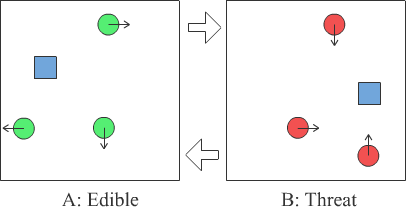
\includegraphics[scale=0.5]{PreyPredatorDomain}
\caption{}
\end{figure}
\subsubsection{Sensors}
All networks have 6 inputs and a minimum of 4 outputs. One input is used for bias. A second input is used for sensing the different task: 1 if enemies are edible and 0 otherwise. The last 4 input is used to sense where the nearest enemy in each direction is located by using the manhattan distance. The distance is clamped between 0 and 100 and divided by 100, so the input span from 0 to 1 - where 0 is close and 1 is far away. The four outputs indicate each direction, and the one output with the highest value is the direction the agent will choose.
\subsubsection{Results}
\subsection{Experiment 3 - Environmental split task (Two Rooms)}
\subsubsection{Domain}
\subsubsection{Results}
\end{document}